\documentclass[]{article}
\usepackage[german]{babel}
\usepackage[utf8]{inputenc}
\usepackage{graphicx}
\usepackage{caption}
\usepackage{subcaption}
\usepackage{lastpage}
\usepackage{epstopdf}
\graphicspath{outdir=/u/mhemmer/Documents/Theses/BachelorArbeit/}
\usepackage{fancyhdr}
\usepackage{amsmath}
\usepackage{amsthm}
\usepackage{amsbsy}
\usepackage{amssymb}
\usepackage{hyperref}


\pagestyle{headings}
\fancyhf{}
\setcounter{section}{-1}								%Gliederungsnummerierung faengt bei 0 an.

%opening
\title{Reduzierung der systematischen Unsicherheit bei der Peakeextraktion neutraler Pionen durch Monte Carlo Template Fits}
\author{Marvin Hemmer}

\begin{document}

\maketitle
\newpage
\tableofcontents
\newpage

	\section{Einleitung}

	\section{Experimenteller Aufbau}

	\section{Analyse}
	\subsection{Daten}
	\subsubsection{Datensatz}
	\subsubsection{Trigger und Cuts}
	\subsection{Peak Extraktion mit der Standard Methode}
	Messungen mit dem EMCal liefern Ort und Energie von u.a. Photonen Kandidaten. Mit diesen Informationen ist es m{\"o}glich neutrale Pionen zu rekonstruieren, da ein ${\it \pi^{0}}$ zu $\left( 98.823\pm0.034\right)\%$ in zwei Photonen zerf{\"a}llt. Der Zerfall findet statistisch Verteilt nach eine Durschnitssl{\"a}nge von ${\it c\tau} = 25.5$nm vom prim{\"a}ren Vertex statt, wobei dieser mit Hilfe der ITS bestimmt.
	Mit dem Wissen, wo sich der prim{\"a}ren Vertex befindet, sowie der Ortsaufl{\"o}sung des EMCals kann der Zerfallswinkel zwischen zwei Photonen Kandidaten, welche durch das EMCal detektiert wurden, bestimmt werden.
	Die Energien der beiden Photonen $E_{\gamma1}$ und $E_{\gamma2}$, sowie der Zerfallswinkel sind f{\"u}r die Berechnung der invariante Masse erforderlich. F{\"u}r diese gilt:
	\begin{align}
	\label{eq_invmass}
	m_{inv} &= \sqrt{2E_{\gamma1}E_{\gamma2}(1-\cos\left( \theta_{\gamma\gamma}\right) )} 
	\end{align}
	Au{\ss}erdem kann aus den vorangegangenen Daten die Aufteilung des Impulses der Photonen Kandidaten bestimmt werden, welche wiederum notwendig ist, um den transversalen Impuls $p_{T}$ des $\pi^{0}$ zu Kalkulieren.
	Es gilt:
	\begin{align}
	\label{eq_pt}
	p_{T\pi^{0}} &= \sqrt{\left(p_{x1}+p_{x2}\right)^{2} +\left(p_{y1}+p_{y2}\right)^{2}} 
	\end{align}
	Die Zahlen in den Indizes beziehen sich dabei auf die Nummerierung der beiden Photonen.
	
	
	\subsubsection{Rekonstruktion}
	\begin{figure}[tbp]
		\centering
		\begin{subfigure}{.5\textwidth}
			\centering
			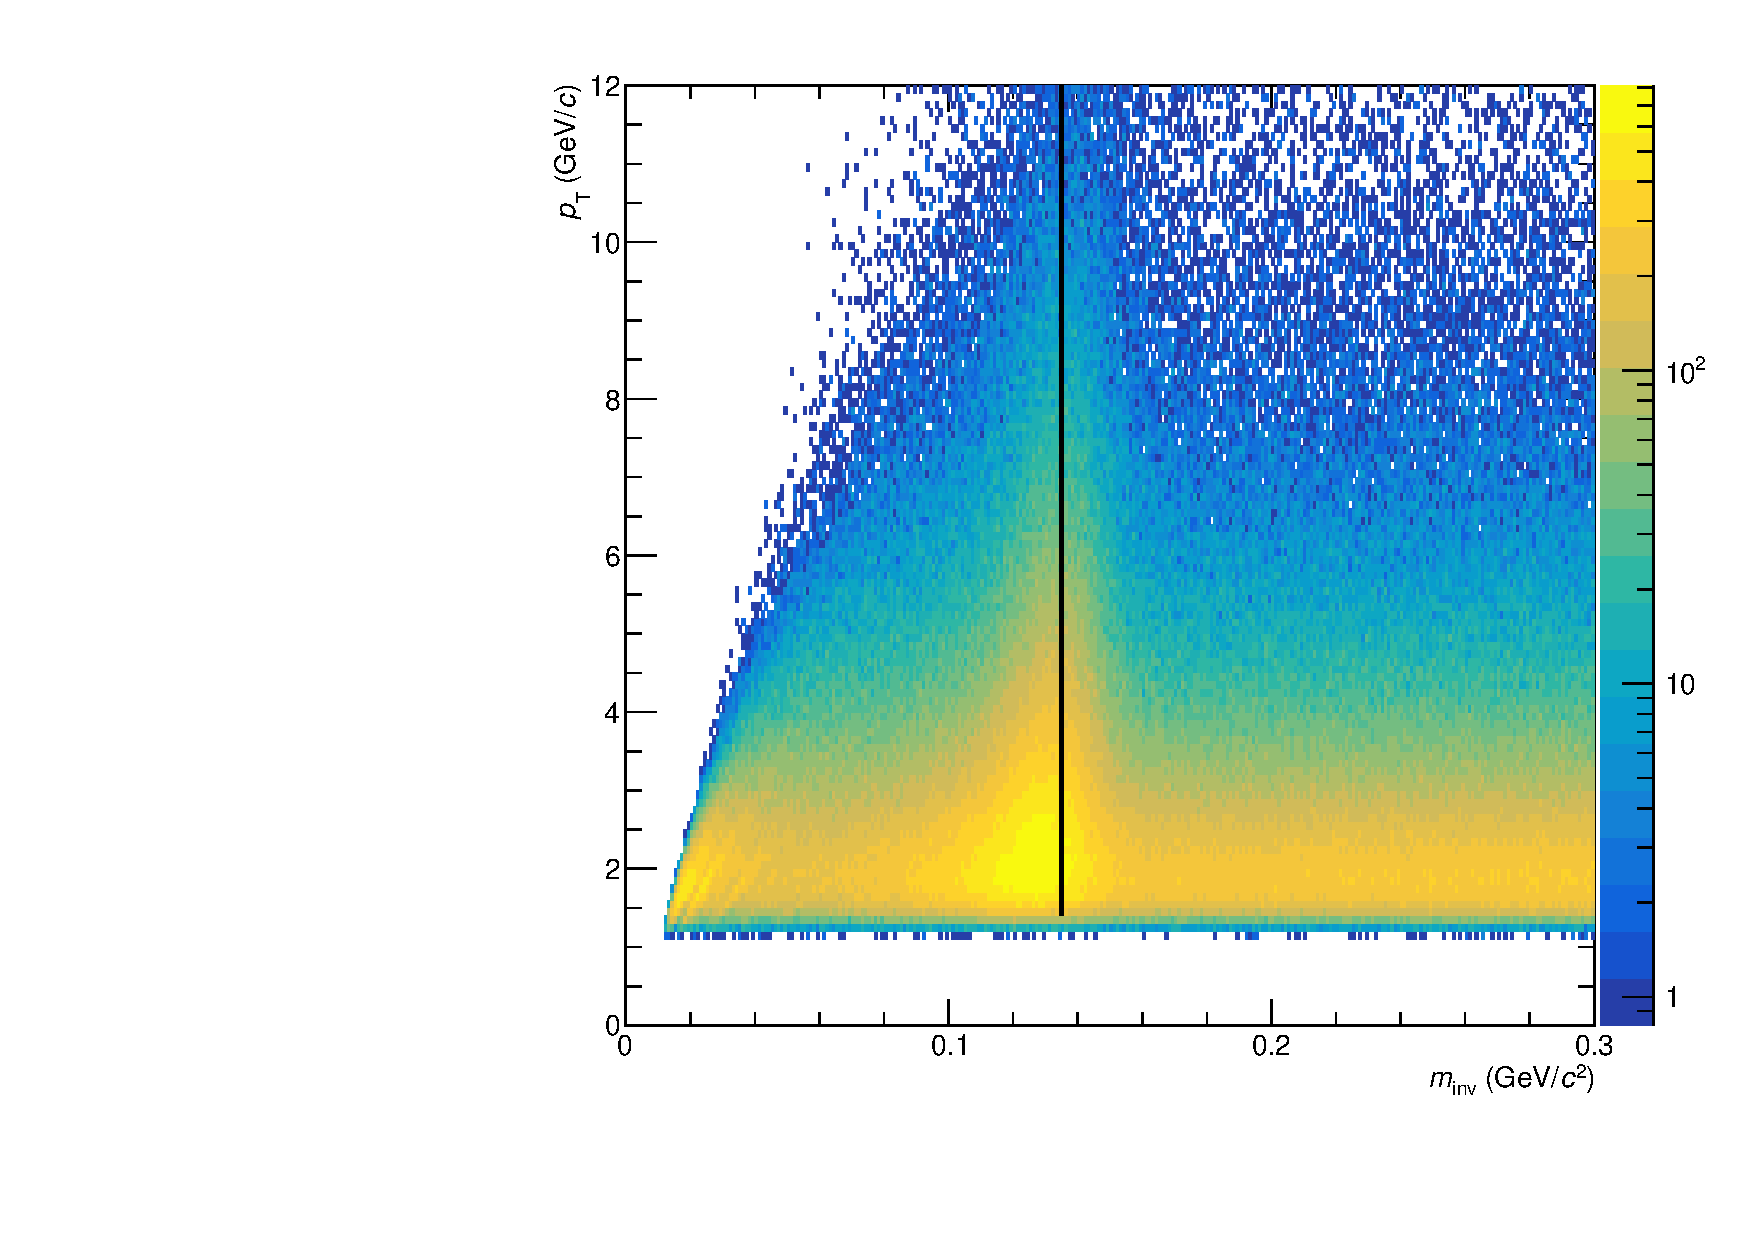
\includegraphics[width=.95\linewidth]{hInvMass_pT_Signal.pdf}
			\caption{}
			\label{figInvMassPt_a}
		\end{subfigure}%
		\begin{subfigure}{.5\textwidth}
			\centering
			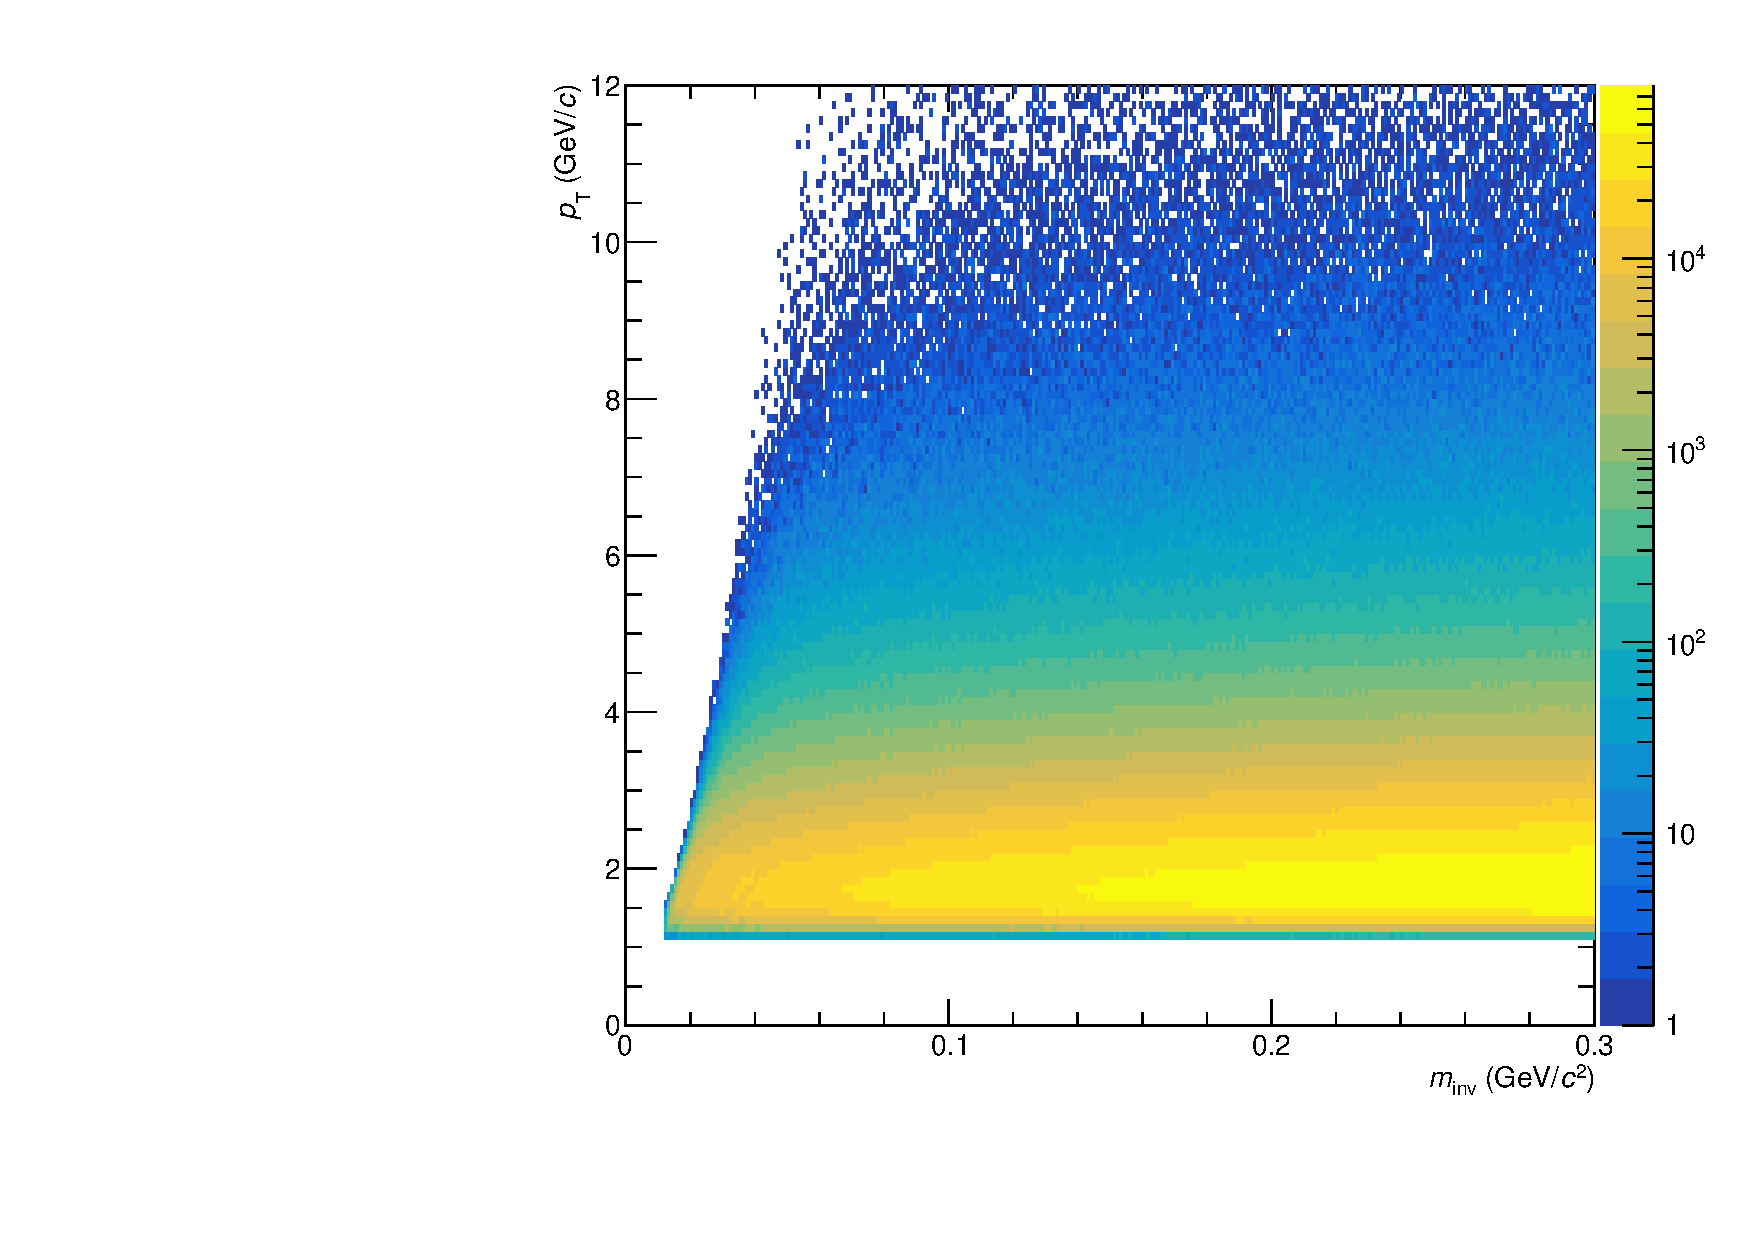
\includegraphics[width=.95\linewidth]{hInvMass_pT_Bkg.pdf}
			\caption{}
			\label{figInvMassPt_b}
		\end{subfigure}
		\caption{\newline{\bf (a)}: Rekombination von Cluster-Paaren aus jeweils der gleichen Kollision ({\it same event}).Die schwarze Linie liegt im Bereich $m_{inv}=0.135\text{GeV/}c^{2}$ was ungef{\"a}hr der $\pi^{0}$ Masse entspricht. Dort ist eine deutliche Peakstruktur zu Erkennen.\newline{\bf (b)}: Rekombination von Cluster-Paaren aus jeweils unterschiedlichen Kollision ({\it mixed event}). Beides in Abh{\"a}ngigkeit der invarianten Masse, sowie des transversalen Impulses.}
		\label{figInvMassPt}
	\end{figure}
	Aus dem gew{\"a}hlten Datensatz werden alle m{\"o}glichen Kombinationen von zwei Photonen Kandidaten aus der gleichen Kollision ({\it same event}) mit korrespondierendem $\theta_{\gamma\gamma}$ benutzt, um $m_{inv}$ nach \ref{eq_invmass} zu berechnen, sowie $p_{T,\pi^{0}}$ nach \ref{eq_pt} und so eine invariante Massenverteilung zu erhalten (vgl. Abbildung \ref{figInvMassPt_a}). In dieser Verteilung ist bereits eine auffallende Struktur bei $m_{inv}\approx 0.135\text{GeV/}c^{2}$ zu erkennen, welche auf richtig rekombinierte $\pi^{0}$ schlie{\ss}en l{\"a}sst. Abbildung \ref{figInvMassPt_b} zeigt eine invariante Massenverteilung bei der Photonen Kandidaten aus unterschiedlichen Kollisionen ({\it mixed event}) miteinander kombiniert werden, auf welche in Kapitel \ref{sssec:num3} genauer eingegangen wird.\newline
	
	\begin{figure}[tbp]
		\centering
		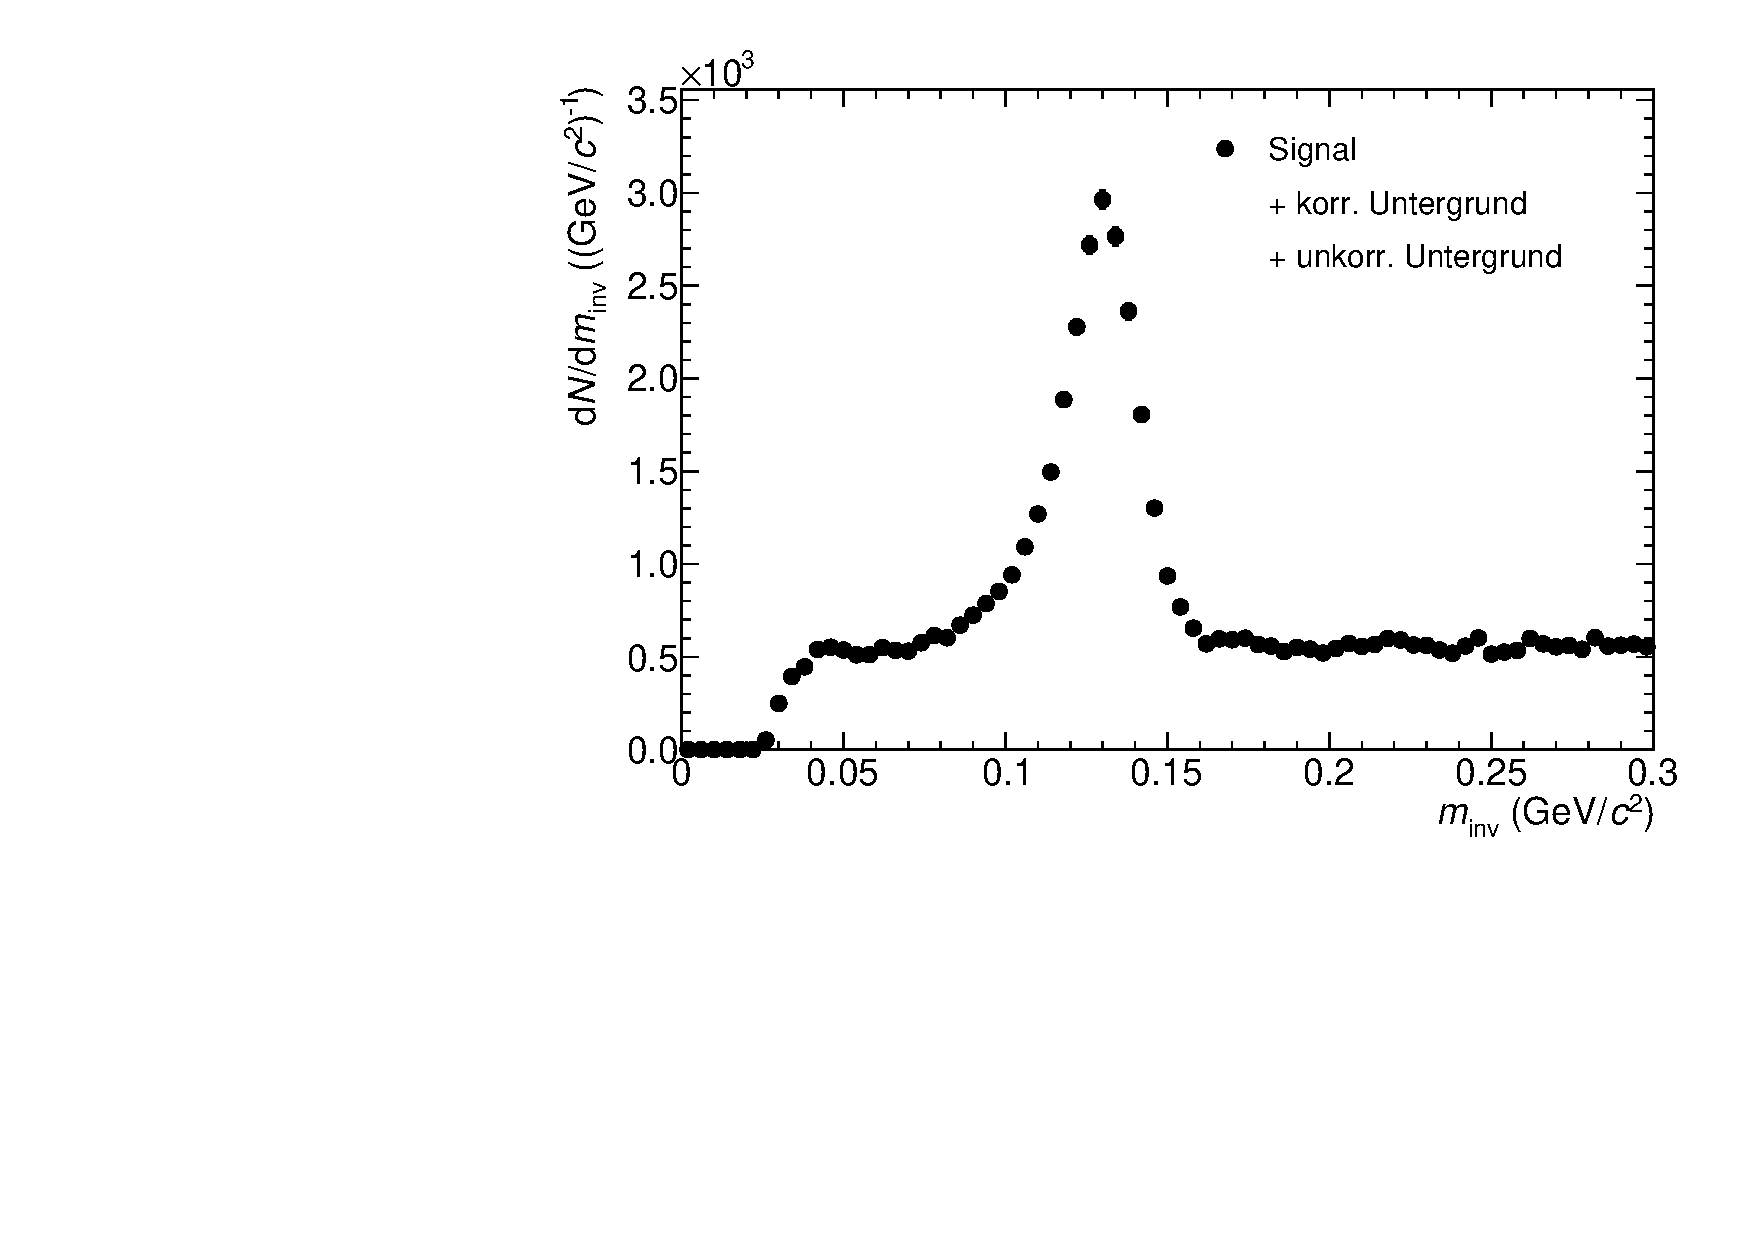
\includegraphics[width=.8\linewidth]{hSignalPlusBkg.pdf}
		\caption{text}
		\label{key}
	\end{figure}
	
	Um $\pi^{0}$s in einzelnen $p_{T}$-Intervallen z{\"a}hlen zu k{\"o}nnen wird die Verteilung in entsprechende Abst{\"a}nden auf die Y-Achse projiziert. Die Intervalle werden so gew{\"a}hlt, dass sie m{\"o}glichst klein sind, w{\"a}hrend die statistischen Unsicherheiten nicht zu gro{\ss} werden. Man erh{\"a}lt Verteilungen der invarianten Masse, welche aus Signal, sowie korreliertem und unkorreliertem Untergrund bestehen. Dennoch ist ein deutlicher Peak im Bereich der Pionenmasse von ca. 135MeV/$c^{2}$ zu erkennen. Um das Signal zu extrahieren werden im Folgende die beiden Komponenten des Untergrunds abgesch{\"a}tz.
	
	\subsubsection{Absch{\"a}tzung des unkorrelierten Untergrunds}
	\label{sssec:num3}
	
	Durch das kombinieren aller Photonenkandidaten ist ein gro{\ss}er Anteil der rekonstruierten Massen nicht korreliert, da die beiden Photonen nicht zusammenh{"a}ngen {\"u}ber beispielsweise einen Zerfall. Um diesen unkorrelierten Untergrund abzuw{\"a}gen kombiniert man im sogenannten Eventmixing Photonen aus unterschiedlichen Events zusammen, da so sicher keine Verbindung zwischen den beiden Photonen besteht.
	
	
	Die Verteilung aus den mixed Events weist keinen Peak auf und hat eine gr{\"o}{\ss}ere Anzahl Eintr{\"a}ge, als die Verteilung aus dem selben Events, weshalb die mixed Event Verteilung an die der same Events skaliert werden muss. Die Skalierung erfolgt im rechten Bereich au{\ss}erhalb des $\pi^{0}$-Peaks und es ergibt sich f{\"u}r den Skalierungsfaktor:
	\begin{align}
	\alpha &= \frac{\sum_{i \neq j}\sum_{n}m_{inv}\left( \gamma^{(n)}_{i},\gamma^{(n)}_{j}\right) }{\sum_{i,j}\sum_{n \neq m}m_{inv}\left( \gamma^{(n)}_{i},\gamma^{(m)}_{j}\right) }
	\end{align}
	Die oberen Indizes stehen hierbei f{\"u}r das Event, aus welchem ein Photon kommt. 
	\subsubsection{Absch{\"a}tzung des korrelierten Untergrunds}
	\subsection{Peak Extraktion mit Templates}
	\subsubsection{Templates}
	\subsubsection{Fit Methode}
	\section{Korrigierter Yield}
	\subsection{Korrekturen}
	\subsection{Variationen}
	\section{Zusammenfassung und Aussicht}



\end{document}
